% !TEX root = main.tex

\section{XXX Model}
To address the above-described challenges, we illustrate XXX, which is first approach~\textcolor{red}{(or system?)} for cryptocurrency transaction graph analysis based on graph embedding.

Fig.~\ref{fig:architecture} depicts the overall architecture of our XXX model. Correlating to the three phases introduced in section~\ref{subsec:methodology}, we explain our model in following three aspects, \emph{preprocessing}, \emph{embedding} and \emph{prediction}.

\begin{figure}[htbp]
	\centering
	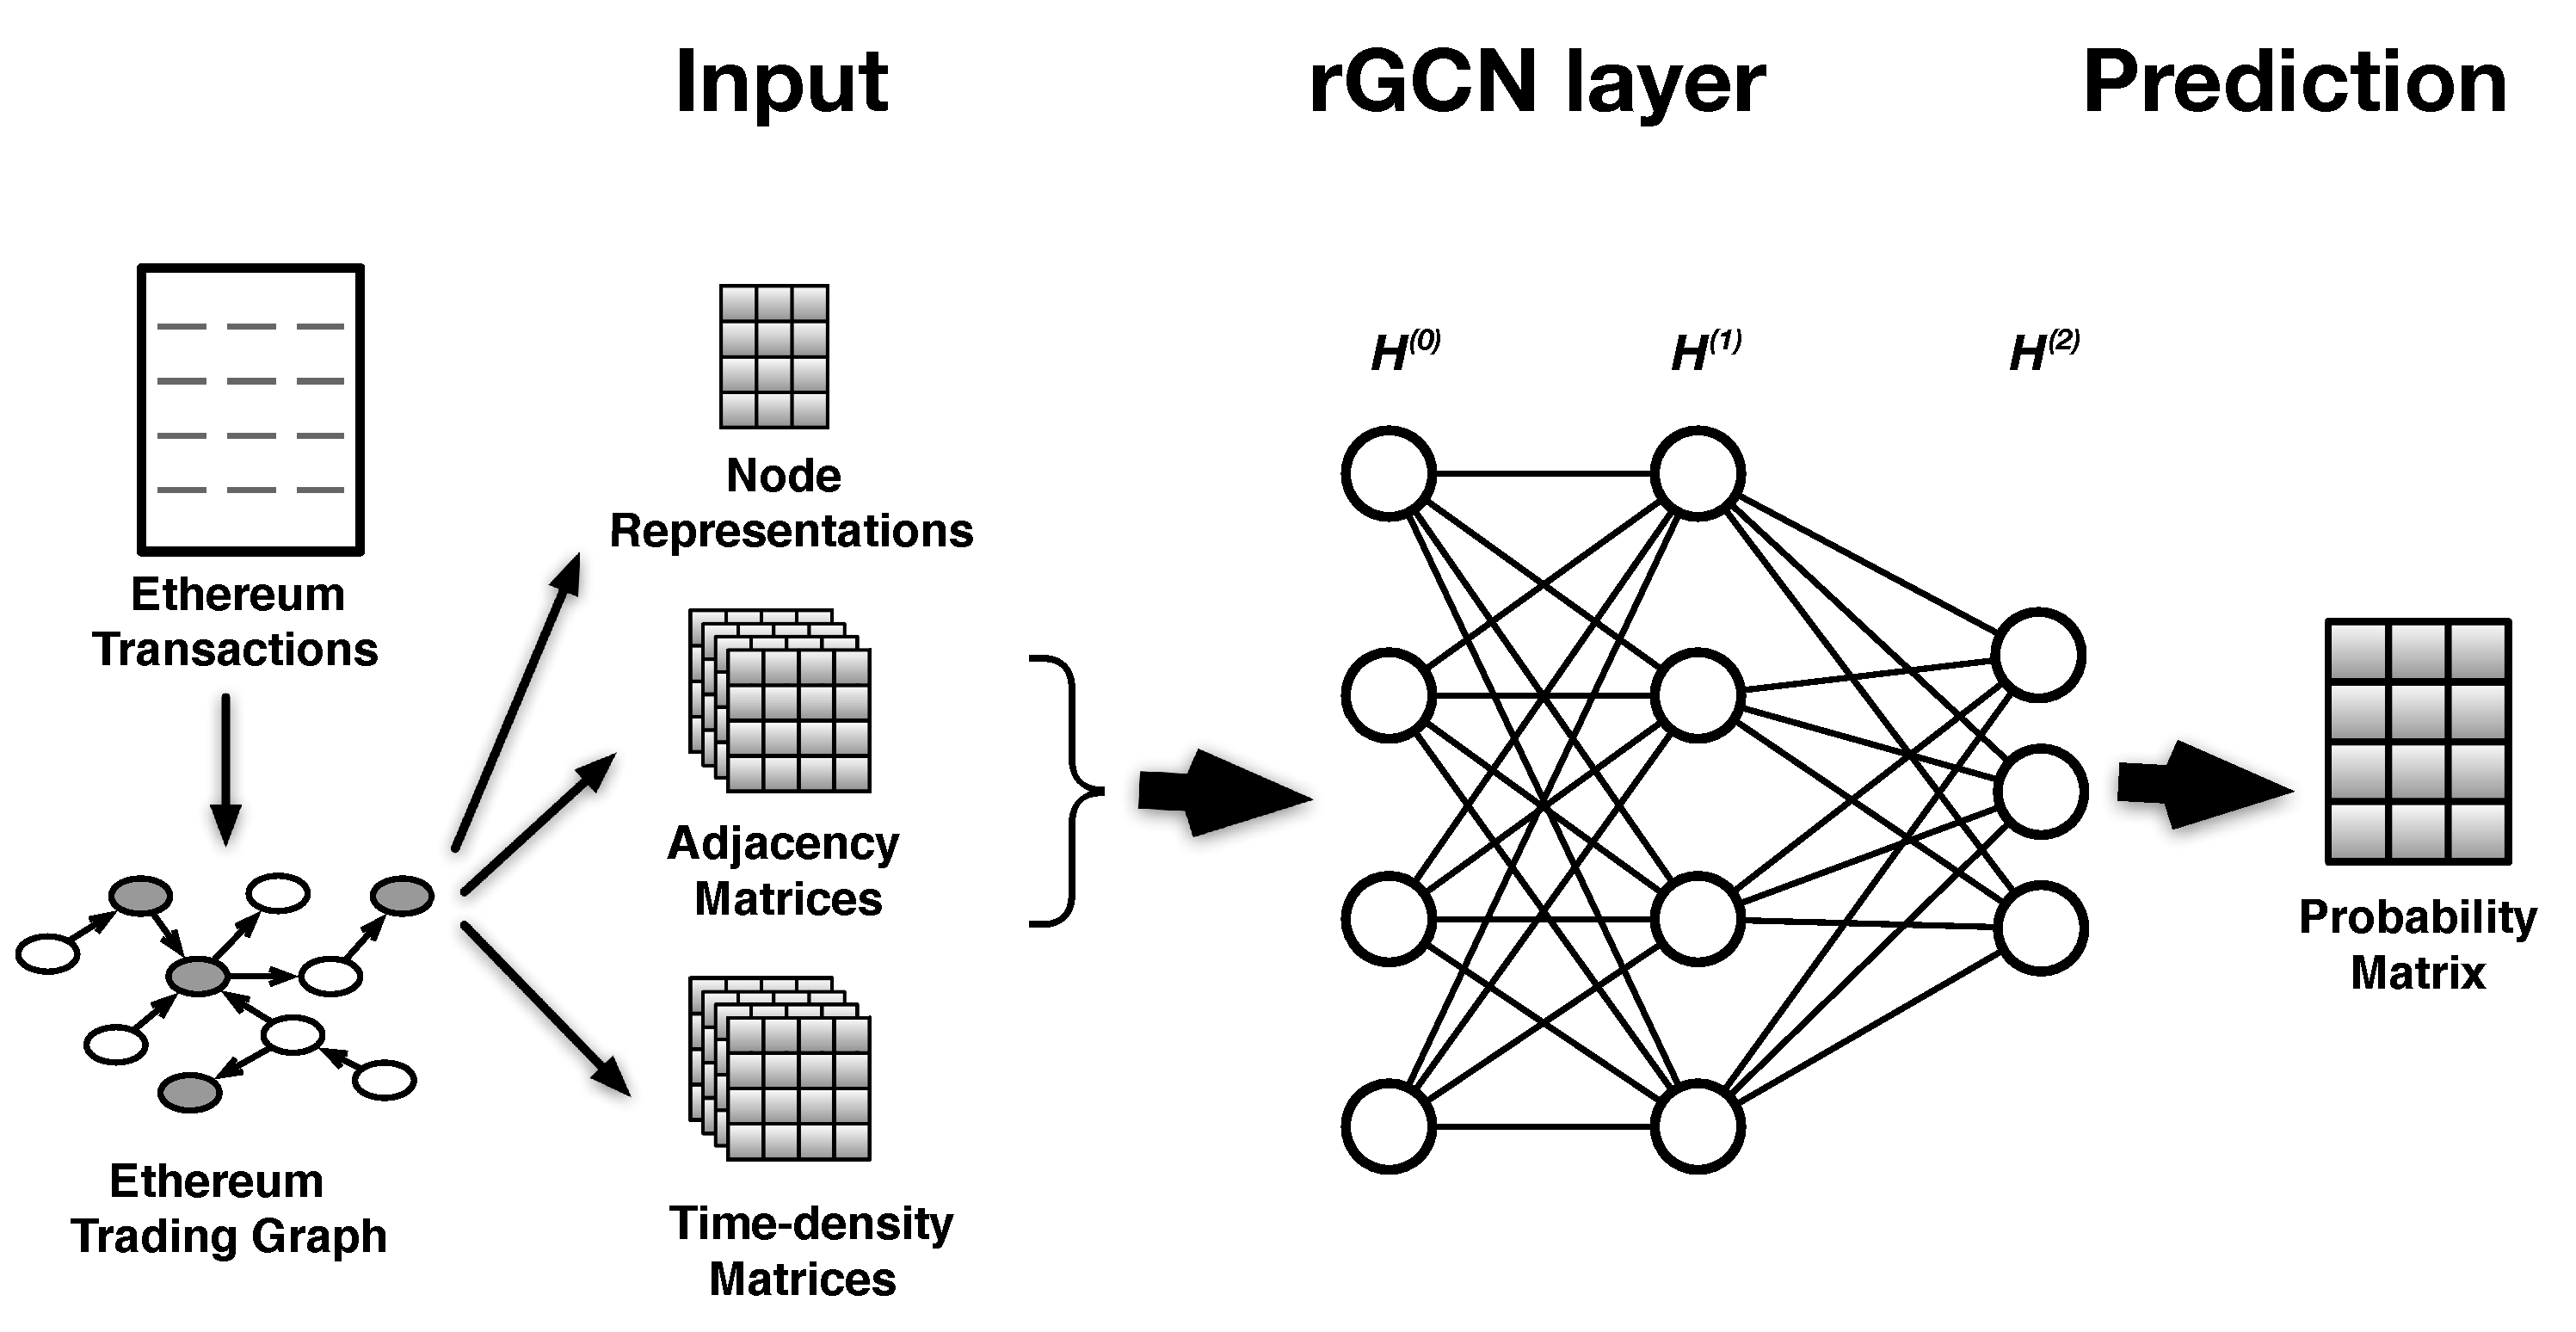
\includegraphics[width=3.5in]{fig/architecture.eps}
	\caption{Overall architecture.}
	\label{fig:architecture}
\end{figure}


\subsection{Preprocessing}
\label{sec:input}
In the preprocessing, the Ethereum transaction graph is constructed based on original transaction logs at first. Different from other studies, the graph is translated to several matrices as the input of embedding model.

 The inputs consist of three parts: (1) a node representation matrix that captures the structural and additional information of accounts, (2) a list of adjacency matrices which describe different relations, and (3) a list of time-density matrices that represent transaction intensiveness between each pair of nodes.

\textbf{Account representations.} We use a feature matrix $X \in \mathbb{R}^{N \times d}$ to encode the overall structural and additional information of each account. The $d$ terms include some pre-defined vectors and here we use the following features
\begin{itemize}
	\item \emph{in-degree}: the number of edges incoming to a node, that is, the number of transactions initialed by an account.
	\item \emph{out-degree}: the number of edges outgoing from a node, that is, the number of transactions which point to an account.
	\item \emph{weighted in-degree}: the summation of all weights of edges incoming to a node, which represents the total Eth received by an account. 
	\item \emph{weighted out-degree}: the summation of all weights of edges outgoing to a node, which represents the total Eth send from an account. 
	%\item eccentricity
	%\item clustering coefficient
	\item \emph{account type}: whether the account is a contract or EOA.
\end{itemize}

%such as in-degree, out-degree, weighted degree, eccentricity, clustering coefficient. Besides, the account type (EOA or SC) is also considered.   

These features help the following layers to pay attention to structural similarity between nodes.

\textbf{Relations.} To investigate the multi-relations in ETG, we divide the raw ETG into different graphs and capture the relations of graph neighboring nodes using adjacency matrices. 

The list of adjacency matrices, $\{A^1,A^2,\dots,A^R|A^i\in \mathbb{R}^{N \times N}\}$ describes the $R$ relations among $N$ nodes in ETG. As we mentioned before, the strategy of division has a large influence on classification performance. 

In our model, the relations are constructed from four categories, including \texttt{CALL} with ETH, \texttt{CALL} without ETH, \texttt{CREATION} and \texttt{REWARD}, which represent the relations of ETH transferring, smart contract invocation, smart contract deployment and mining rewarding. 

We consider the 4 types of forward transactions introduced above and 4 reverse relations in order to pass information from the opposite direction. Besides, a self loop as a special relation type is included to retain information of the previous layer in the GCN network. 

For contract invocation, contract deployment and mining rewarding relations, we calculate the frequency of repeated edges between a nodes pair as the adjacent weight in the corresponding relation adjacency matrix. For ETH transferring, on the other hand, it is not sensible to use the amount of ETH flow directly as the adjacent weight. That is because the accounts have varied enormously in terms of ETH transferring which \textcolor{red}{will lead to underflow and overflow in the process of training.} Here the amount of ETH transferring is discretized into (1) small transfers which the transaction value is less than 1 ETH; (2) medium transfers which the transaction value is between 1 ETH and 10 ETH and (3) major transfers which the transaction value is above 10 ETH. Then the ETH transferring matrix can be calculate as well as the former relations.

Specially, the adjacency matrices are modified to preserve the asymmetric proximity of ETG, which will be addressed in detail later. 

\textbf{Time-density matrices.} We also find that the relationship between a pair of nodes differs from another, even they have the same transaction frequency or adjacency weight. This insight inspire us to use time-density information.

Correlated to the adjacency matrices, a list of time-density matrices $\{K^1,K^2,\dots,K^R|K^i\in \mathbb{R}^{N \times N}\}$ describes the concentration of relations. 

Given a sequence $\{h_{ij1}^r,h_{ij2}^r,\dots,h_{ijm}^r | h_{ijk}^r>0\}$ as the block height of transactions in relation $r$ between node $v_i$ and $v_j$. The time-density of each relation $r$ is computed as%Equation \ref{eq:time}

\begin{equation}
k_{ij}^r=g(\sqrt{Var[\frac{1}{m}\sum_{k=1}^m h_{ijk}^r]})
\label{eq:time}
\end{equation}

\noindent where $g(\cdot)$ is the function of squash which can be logarithmic function.

\subsection{Embedding}
\label{sec:rGCN layers}
 We feed the input into GCN based model with 2 hidden layers, as a trade-off between preserving high-order proximities and introducing noise.

The input to rGCN $l$-th layer is defined as $H^{(l)}={h_1^{(l)},h_2^{(l)},...,h_N^{(l)}|h_i^{(l)}\in \mathbb{R}^{N \times d^{(l)}}}$.

%In raw rGCN model, the propagation model can be expressed as
%\begin{equation}
%h_i^{(l+1)}=\delta(\sum_{r\in R} \sum_{j \in N_i^r} \frac{1}{c_{i,r}}W_r^{(l)}h_j^{(l)}+W_0^{(l)}h_i^{(l)})
%\label{eq:rgcn}
%\end{equation}
%\noindent where $r \in R$ represents a kind of relation, $N_i^r$ denotes the set of neighbor indices of node $v_i$ under relation $r$, and $c_{i,r}=\frac{1}{|N_i^r|}$. Single self-connection is also introduced as a special relation type to each node. %compared with Eq.\ref{eq:gcn}The node feature $h_i$ is updated as:

To 

We improve the forward updating process of raw rGCN as 
\begin{equation}
h_i^{(l+1)}=\delta(\sum_{r\in R} \sum_{j \in N_i^r} \frac{\tau_{ij}^r}{\hat c_{i,r}}W_r^{(l)}h_j^{(l)})
\end{equation}

\noindent where $r \in R$ represents a kind of relation, $N_i^r$ denotes the set of neighbor indices of node $v_i$ under relation $r$, and $\tau_{ij}^r$ is the time-density of transactions from node $v_i$ to $v_j$. 

The coefficient $\hat c_{i,r}$ is computed as:
\begin{equation}
\hat c_{i,r}=\frac{1}{d_i^r\cdot |N_i^r|}
\end{equation}

\noindent where $d_i^r=\sum_{j}A^r_{ij}$, preserving the asymmetric proximity, and $|N_i^r|$ plays the role of normalization.

The method can be understood as a more abstract propagation rule:
\begin{equation}
H^{(l+1)}=\delta(\sum_{r\in R} (K^r\odot (D^r)^{-1}A^r)H^{(l)}W_r^{(l)})
\end{equation}
\noindent where $H^{(l)}$ is the matrix of activations in the $l$-th layer, and $H^{(0)}=X$. $\delta(\cdot)$ denotes an activation function such as the ReLU$(\cdot)$ = max$(0,\cdot)$. $D^r$ is a diagonal matrix where $D^r_{ii}=\sum_{j}A^r_{ij}$. $\odot$ indicates point-wise multiplication.

\subsection{Prediction and Training}
The output of the last layer indicates the probability that each point being assigned to each class.

The output of the last rGCN layer is regarded as a probability matrix $P=\{p_1,p_2,...,p_N|p_i\in \mathbb{R}^{N \times m}\}$, where $p_i=\{p_{i,1},p_{i,2},...,p_{i,m}\}$ describes the probability of classifying node $v_i$ into $m$ categories. 

We utilize the cross-entropy loss function as the training objective:
\begin{equation}
L=-\sum_{i=1}^T\sum_{j=1}^m y_{i,j}\log p_{i,j}+\lambda ||\theta||^2
\end{equation}

\noindent where $T$ is the number of training samples, $y_{i,j}$ is the true probability of node $v_i$ belonging to category $j$. $\theta$ is the set of all parameters and $\lambda$ is the coefficient for $L_2$  regularization.
